% Exmaple thesis using jthesis class
% Written by George Taylor (gstaylor@iee.org)
%
% Please mail all comments and changes to G.S.Taylor@ee.ed.ac.uk
% so that this package can be kept up to date.

\typeout{PhD Thesis class example}

% Supported options to jthesis:
%	nohyphens 		make hyphenation incredibly unlikely
%				(the university guidelines suggest this)
%				if you get an awakward line you will need
%				to either change it, or use \-
%
%	doublespace		double space eveything except
%				contents, lists of figures etc and references
%				Personally I think double spacing sucks.
%				Use \begin,end{singlespace} for exceptions.
%				(safe to use even when doublespace option
%				 not given)
%
% Other options (not part of jthesis) which you may wish to use:
% twoside - for two sided output
% fleqn - left indented (rather than centered) equations
%
\documentclass[doublespace]{StyleFiles/jthesis-v1}

% By default a eps file of the University Crest is assumed to be
% in the StyleFiles directory. However you may wish to give a full
% absolute pathname here so that xdvi, dvips etc work even when run
% from another directory.
%\crestfile{/home/gst/PhD/Thesis/StyleFiles/EdUniCrest.eps}

% The array package extends tabular, for example useful for <{$},>{$}
% when using tables of symbols
\usepackage{natbib}
\usepackage{array}

% It is recommended you use amsmath for better looking equations,
% but the jthesis class does not enforce this.
\usepackage{amsmath}

% Use subfigure to put multiple figures into one - complete with
% mini captions.
%\usepackage{subfigure}
\usepackage{subfig}

% Other useful packages you might not otherwise find out about:

\usepackage{booktabs}
% \usepackage{psfrag}	% replace labels in xfig diagrams with nice math
% \usepackage{endfloat} % put all floats at end
% \usepackage{shadow}   % for shadowed boxed round things
% \usepackage{bar}	% for bar charts
% \usepackage{draftcopy} % prints DRAFT across each page in big grey letters
% \usepackage{mathtime}  % for times font style maths (may require some fonts)
% see also the documentation for the graphicx package providing
% support for postscript images and colour (already \usepackage'd)

\usepackage{dcolumn}
\usepackage{hyperref}
\usepackage{tabularx}
\usepackage{lscape}
\usepackage{graphicx}
\usepackage{rotating}

% Tip: If you include your own .sty/.cls files with \usepackage
% instead of \include separate .aux files will not be generated for
% each included file.
%\usepackage{StyleFiles/mymacros}


% Tip: use \includeonly to only include one thing and ignore all other
% \include commands, this is handy for formatting only one chapter
% at a time
%\includeonly{Chapter1/chapter1}


\begin{document}

% Put your title, your name, and submission date here
% use \date{} if you don't want a date, todays date is used
% if \date is omitted.
\title{My Very interesting Thesis}
\author{Sam Hawkins}
\date{September 2010}

\maketitle

% If you look in the included files you will notice the use of
% \minorchapter.

\include{Preliminary/abstract}
\include{Preliminary/declaration}
\include{Preliminary/acknowledgements}

% Insert table of contents and lists of figures and tables.
\contentsandlists

% More use of minorchapter
\include{Preliminary/abbreviations}
\include{Preliminary/nomenclature}

% \startchapters indicates the main chapters follow, this changes
% things such as the page numbering.
\startchapters

\chapter{Some Simple Text}

\section{Using some `natbib' Citations}

The following paragraph demonstrates some simple text with some citations. The
command
\begin{verbatim}
\citep[see][]{bibtex:key}
\end{verbatim}
puts a citation in parathesis with the word `see' before the follows easily.
reference itself. The second optional `[~]' puts something after the reference,
such as `chapter 3' as seen \cite{Glover.2012} in the second citation in the paragraph \cite{Grainger.1994}. Also the
command \cite{Jenkins.2000}
\begin{verbatim}
\citet[]{bibtex:key}
\end{verbatim}
will produce an inline citation, i.e., not in parenthesis. Note that a blank
line must be places between paragraphs \index{Fourier Series}in the raw latex, e.g.
\begin{verbatim}
Some text in first paragraph.

Some text in second paragraph.
\end{verbatim}

At the beginning of this, I'd like to add a reference by
as it has a junior in it and it's good to see how that formats. Pellentesque id
mi sit amet mauris elementum sagittis eget at neque. Quisque id sapien magna, et
pharetra enim. Aenean congue turpis et libero faucibus vitae vulputate erat
facilisis. Pellentesque iaculis orci a nisl scelerisque quis accumsan sem
viverra. In nec risus dolor, vitae adipiscing erat
pellentesque id mi sit amet mauris elementum \index{Abernathy}
sagittis eget at neque. Proin tincidunt sollicitudin sagittis. Pellentesque id
mi sit amet mauris elementum sagittis eget at neque. Quisque id sapien magna, et
pharetra enim. Aenean congue turpis et libero faucibus vitae vulputate erat
facilisis. Pellentesque iaculis orci a nisl scelerisque quis accumsan sem
viverra. In nec risus dolor, vitae adipiscing erat
pellentesque iaculis orci a nisl scelerisque
quis accumsan sem viverra. In nec risus dolor, vitae adipiscing erat.

\section{Entering and Referencing a Figure}

The next paragraph demostrates a reference to a figure and then a the figure
itself. Note the standard layout for a figure is
\begin{verbatim}
\begin{figure}[htb] % htb is positional preference (here, top, bottom)
  \centering
  \includegraphics[width=some width]{filename without extension}
  \caption{Caption Title}
  \label{fig:label}
\end{figure}.
\end{verbatim}
The reference to the figure is then provided by something like
\begin{verbatim}
figure~\ref{fig:label}.
\end{verbatim}

Lorem ipsum dolor sit amet, consectetur adipiscing elit. Pellentesque id mi sit
amet mauris elementum sagittis eget at neque. Quisque id sapien magna, et
pharetra enim. Aenean congue turpis et libero faucibus vitae vulputate erat
facilisis. Pellentesque iaculis orci a nisl scelerisque quis accumsan sem
viverra. In nec risus dolor, vitae adipiscing erat. Etiam ultrices leo eget arcu
faucibus congue. Nullam eget iaculis mauris. Ut gravida rutrum nisl eget auctor.
Donec sodales enim at massa porta nec mattis est dapibus. Nunc nec vehicula
tellus. Quisque massa tellus, lobortis vel sodales sed, aliquet varius dui.
Proin tincidunt sollicitudin sagittis. Figure~\ref{fig:bottomkutta} shows
something unrelated to this paragraph, but neatly demonstrates how to stick a
figure in and reference it.

\begin{figure}[htb]
  \centering
  %% Because graphicspath was set in edengths.tex you only need to
  %% supply the file name here, i.e. examplepicture (doesn't need the
  %% extension) and not the full path. Just remember to add the path
  %% to \graphicspath{{thispath/}{thatpath/}}
  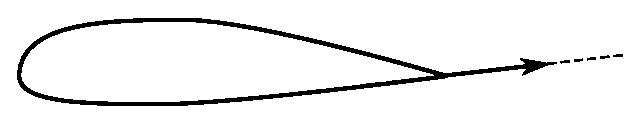
\includegraphics[width=0.3\textwidth]{bottomkutta}
  \caption{Alternative orientations of the wake vortex sheet as it separates
  from the trailing edge of the aerofoil.}
  \label{fig:bottomkutta}
\end{figure}

\section{Quoting Something}

The final paragraph in this chapter illustrates a quote. To do a quote
simply use the enviroment
\begin{verbatim}
\begin{quote}
 The quote text.
\end{quote}.
\end{verbatim}
Note that the edengths class forces quotes to single spacing as the thesis
regulations demand this. Also, there is an inline citation in the next
paragraph.

Lorem ipsum dolor sit amet, consectetur adipiscing elit. Pellentesque id mi sit
amet mauris elementum sagittis eget at neque. Quisque id sapien magna, et
pharetra enim. Aenean congue turpis et libero faucibus vitae vulputate erat
facilisis. Pellentesque iaculis orci a nisl scelerisque
quis accumsan sem viverra. In nec risus dolor, vitae adipiscing erat. Etiam
ultrices leo eget arcu faucibus congue. Nullam eget iaculis mauris. Ut gravida
rutrum nisl eget auctor. Donec sodales enim at massa porta nec mattis est
dapibus. Nunc nec vehicula tellus. Quisque massa tellus, lobortis vel sodales
sed, aliquet varius dui. Proin tincidunt sollicitudin sagittis. 
\begin{quote}
 ``Lorem ipsum dolor sit amet, consectetur adipiscing elit. Pellentesque id mi
sit amet mauris elementum sagittis eget at neque. Quisque id sapien magna, et
pharetra enim. Aenean congue turpis et libero faucibus vitae vulputate erat
facilisis.''
\end{quote}
Lorem ipsum dolor sit amet, consectetur adipiscing elit. Pellentesque id mi sit
amet mauris elementum sagittis eget at neque. Quisque id sapien magna, et
pharetra enim. Aenean congue turpis et libero faucibus vitae vulputate erat
facilisis. Pellentesque iaculis orci a nisl scelerisque quis accumsan sem
viverra. In nec risus dolor, vitae adipiscing erat. Etiam ultrices leo eget arcu
faucibus congue. Nullam eget iaculis mauris. Ut gravida rutrum nisl eget auctor.
Donec sodales enim at massa porta nec mattis est dapibus. Nunc nec vehicula
tellus. Quisque massa tellus, lobortis vel sodales sed, aliquet varius dui.
Proin tincidunt sollicitudin sagittis. 

\chapter{Another Chapter}

\section{The first section}

Note that all section and chapter titles should use lower case except
for the first character of the first word. Here is a reference to a
paper~\cite{apaper}. Figure~\ref{fig:picture} is a weird picture.

\begin{figure}[h]
  \centering
  %% Because graphicspath was set in edengths.tex you only need to
  %% supply the file name here, i.e. examplepicture (doesn't need the
  %% extension) and not the full path. Just remember to add the path
  %% to \graphicspath{{thispath/}{thatpath/}}
  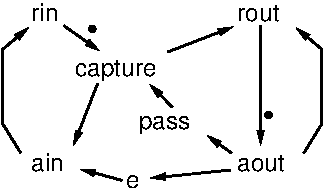
\includegraphics[width=2in]{examplepicture}
  \caption[Long caption and \textit{some italics} to see what happens]%
  {This is an example of pdf with a very long caption and \textit{some italics} to see what happens and it should see what happens over two lines.}
\label{fig:picture}
\end{figure}

\subsection{A subsection}

Lorem ipsum dolor sit amet, consectetur adipiscing elit. Maecenas nec orci lacus, ac sollicitudin tortor. Maecenas rutrum vestibulum rhoncus. Vestibulum non ligula nibh. Cum sociis natoque penatibus et magnis dis parturient montes, nascetur ridiculus mus. Phasellus egestas sodales lacus, ac scelerisque nulla venenatis sed. Ut elementum turpis ac lacus consectetur consequat. Sed at est eros. Praesent erat velit, dictum id adipiscing eu, ultrices vel nisi. Nullam at nisl ut est posuere commodo tincidunt eget nisl. Integer id erat non metus adipiscing dignissim quis sed enim. Curabitur viverra lobortis eleifend. Proin vestibulum nunc eu augue dapibus quis porttitor ipsum rhoncus. Duis tortor tellus, suscipit sit amet ornare id, lacinia sed lacus. Ut in molestie ligula. Praesent euismod lectus vitae arcu malesuada tempus. Aliquam pharetra tincidunt augue in eleifend. Curabitur porttitor vulputate quam, ut fringilla mauris porta eu. Curabitur sodales, felis non vestibulum feugiat, urna diam bibendum purus, ac scelerisque massa eros sit amet ipsum. In elementum laoreet aliquam.

\subsubsection{A subsubsection}

Aliquam eget sapien tellus, sed rutrum leo. Vestibulum et quam sit amet dolor gravida sagittis. Aenean dapibus urna a nibh sollicitudin pharetra. Sed nisi augue, vehicula sed tristique facilisis, lacinia ut augue. Nam quis tempor mi. Vestibulum lorem leo, aliquet at sollicitudin vitae, fringilla id odio. Aenean a orci odio. Mauris tincidunt eros ac libero suscipit molestie. Donec feugiat turpis a urna suscipit in pellentesque magna pretium. Vivamus eget nunc vitae nunc ultricies tincidunt. Duis dictum eros et lorem auctor id ullamcorper diam commodo. Pellentesque quis dolor nec urna vestibulum pellentesque. Donec luctus mi ut nisi hendrerit pulvinar. Donec fringilla, lectus vitae accumsan sollicitudin, sem metus mollis risus, nec laoreet ante arcu ut augue.

\subsection{Another subsection}

Table~\ref{tab:atable} is an example of a~\footnote{this is a
footnote} simple table.

\begin{table}[htb]
\begin{center}
\begin{tabular}{|c|c|c|}
\hline
1.0 & 2.0 & 3.0 \\
\hline
4.0 & 5.0 & 6.0 \\
\hline
\end{tabular}
\caption{A table}
\label{tab:atable}
\end{center}
\end{table}


\section{Another section}

This is a long and boring paragraph for the purpose of testing the
spacing between paragraphs and the use or otherwise of indentation. I
think a space between paragraphs and without the first line indented
is somewhat easier to read than no space between paragraphs and with
the first line indented.

Another equally exciting paragraph, one two three four five six seven
eight nine ten eleven twelve thirteen fourteen fifteen sixteen
seventeen eighteen nineteen twenty and so on.

\begin{equation} \label{eqn:dct}
z(k,l) = \frac{2}{N} \alpha(k) \alpha(l) \sum_{m=0}^{N-1} \sum_{n=0}^{N-1}
         x(m,n) \cos \frac{ (2m+1) \pi k}{2N} \cos \frac{ (2n+1) \pi l}{2N}
\end{equation}

\begin{equation} \label{eqn:idct}
x(m,n) = \frac{2}{N} \sum_{k=0}^{N-1} \sum_{l=0}^{N-1}
         \alpha(k) \alpha(l) z(k,l)
\end{equation}

\begin{quotation}
This is a quotation, another equally exciting paragraph, one two three
four five six seven eight nine ten eleven twelve thirteen fourteen
fifteen sixteen seventeen eighteen nineteen twenty and so on. Just
checking it is single spaced.
\end{quotation}

\include{Chapter3/chapter3}
\include{Chapter4/chapter4}
\include{Chapter5/chapter5}
\include{Chapter6/chapter6}


% \appendix indicates from now on \chapter generates an appendix
% rather than a normal chapter.
\appendix

%\include{Appendix/appendixA}

% \insertreferences inserts the list of references using the IEEE style
% and updates the table of contents. The single argument is a comma
% spearated list of .bib files (just as in \bibliography)
\insertreferences{References/library}

% that's all folks!
\end{document}








